% \newpage
% \thispagestyle{empty}
% \mbox{}
\cleardoublepage

\ifdefined\included
\else
\setcounter{chapter}{1} %% Numéro du chapitre précédent ;)
\dominitoc
\faketableofcontents
\fi

\chapter{A Human-Aware Task Planner able to Emulate Human Decisions and Actions (HATP/EHDA)}
\chaptermark{HATP/EHDA}
\label{chap:2}
\minitoc

\chapabstract{This chapter presents the HATP/EHDA task planner. 
This approach aims to clearly distinguish between the uncontrollable human and the controllable robot agents. Most importantly, it models the distinct human decisional processes and beliefs to be able to reason on it while planning the robot's action.
This planner has been the keystone of most of my work. Hence, the reader should understand the motivation and methods of this task planner.}

\section{Introduction}

I was introduced to task planning with the work of a PhD student from my lab, Guilhem Buisan. I slightly contributed to the original version and then proposed two extensions of his work. However, Guilhem mainly designed and implemented this novel \textbf{H}uman-\textbf{A}ware \textbf{T}ask \textbf{P}lanning approach dedicated to \acrfull{hri}, which plans the robot's actions while estimating and \textbf{E}mulating the \textbf{H}uman \textbf{D}ecisions and \textbf{A}ctions, namely \textbf{HATP/EHDA}. 

We believe this planning approach suits the needs of \acrshort{hri} scenarios well. Thus, it became a laboratory to address relevant challenges of task planning for \acrshort{hrc}. 
Two of my main contributions include addressing such challenges and implementing the solutions as extensions of HATP/EHDA.   
Consequently, it is essential to understand this work's motivation and methods well before introducing my proper contributions. This section introduces, motivates, and explains the HATP/EHDA approach as a background to the other chapters. 
A detailed description of this prototypical planner is already given in Buisan's thesis~\cite{thesisBuisan21}. Thus, large parts of this section are directly retrieved from Buisan's thesis, but they are essential to have in mind. Some notations are adapted to match the descriptions of my contributions in the following chapters. 

\section{A Hierarchical Agent-Based Task Planner (HATP)}

My work and \acrshort{hatpehda} are part of a line of work that started with the \acrfull{hatp} \cite{alili2009task,lallement2014hatp}.

Based on \acrfull{htn}, this planner can elaborate a multi-agent plan based on a single HTN tree. Moreover, it maintains one belief base per agent, allowing the writer to write task decomposition rules and action preconditions and effects in any agent belief base. This approach produces a joint plan that includes actions from all involved agents. 

To make \acrshort{hatp} suitable to \acrshort{hri} scenarios, specific mechanisms to compute costs and filter plans have been included. To this end, \acrshort{hatp} allows balancing efficiency, wasted time, agent effort, intricacy, and undesirable states or sequences. This way, social rules can be defined to produce a collaborative plan that humans will likely accept. 

However, \acrshort{hatp} assumes a shared goal has been established between humans and robots before planning. It is also based on the fact that the generated plan will be shared with and accepted by humans before execution. Indeed, HATP does not represent humans as agents having separate decision-making processes that may lead to diverging plans without robot communication. Hence, any human deviation from their generated stream of action needs supervision to perform repair action or request a replanning. Such an approach can work well, but it assumes that communication can easily be done at any point in the plan. However, this assumption is not always verified for various reasons, \textit{e.g.} noisy environments, making communication costly.
Additionally, any human deviation, \textit{e.g.} due to inattention, will put the robot in a failure state, which needs to be fixed before continuing (replanning).

\section{Rationales of the HATP/EHDA Approach}

The \acrshort{hatp} approach produces what is estimated to be the best joint plan for solving the task. Hence, this approach assumes that humans will likely accept and follow the produced plan. This approach leaves no room for online human decisions and assumes a fully committed human through a previously established shared goal. This approach also considers one shared task representation and knowledge base. To cater to the limitations of \acrshort{hatp}, I participated in the development of a new approach, HATP/EHDA, which tries to satisfy several objectives: 
\begin{enumerate}
    \item \textbf{Plan without assuming a prior shared goal.} In \acrshort{hri} scenarios, the robot and the human do not always share a goal. The robot can, for example, plan to perform a task around humans that are not involved at first, or it may be requested by a human to do a task without wanting to take part in it. HATP/EHDA can balance between integrating the sharing of a goal with a human (assumed to be collaborative) in the plan and making the robot do the task alone or integrating the eventuality to ask for punctual human help. 

    \item \textbf{Model the human decision processes.} When taking part in a task, a human (assumed willing to collaborate with the robot) will also plan to reach their (potentially shared) goal. HATP/EHDA must be able to account for this to provide plans that are expected and explainable by the human partner.

    \item \textbf{Help the human decisions, but not compel them.} Unlike \acrshort{hatp}, HATP/EHDA should account for human decision-making flexibility. While modeling the human decision processes, it is possible to narrow down the possible human actions, and the generated plans must help the supervision (execution of the plan) avoid replanning or repairing during the execution by considering several human actions.

    \item \textbf{Model the potential human reactions.} It is possible to predict that the human may react to some situations, interrupting or helping their current task. Two causes have been identified for these reactions. First, they can result from specific world states humans perceive and interpret. Then, they can also originate from explicit communications issued by the robot. These communications can either be a belief alignment, updating the human knowledge and impacting their decisions, a request to perform a specific action, or a request to help the robot with a shared goal, needing the human to plan for it.

    \item \textbf{Act and decide on the different agents' beliefs.} It is crucial to be able to represent actions as having different effects on the beliefs of the robot or the human. Indeed, some robot actions are partially or not observable by humans; humans cannot know the complete new world state when performing them. Besides, these effects and their observability often depend on the current world state, whose representation must be supported by the planner. Then, planning decisions may require reasoning on both the robot's and human's beliefs. This is especially true with communication actions aiming to align knowledge or ask questions. Finally, some actions of pure decision have no direct effect on the world but only on the internal beliefs of the agents. For example, observation actions will only update the beliefs of the agent doing it.

    \item \textbf{Decide not only on the world state but also on the decision processes of the agents.} Some decisions made during the planning process require access to the agents' beliefs representing the world state and the estimation of their planning processes. For example, the decomposition of a task by the robot may be impossible if some other task is already performed in its partial plan. Other decisions may also need the estimation of the current human planning process. For example, if it were estimated earlier in the plan that the human would perform a specific task decomposition, the planner would assign a complementary task to the robot.

    \item \textbf{Adapt to the human experience, trust, and preferences.} We also want the planning process to be adjusted depending on the actual human it is planning with. It must perform its planned search differently, whether the human has the habit of performing this particular task with the robot or not. Moreover, the human model can be adjusted to the human's trust in the robot and their preferences.

\end{enumerate}

\section{Related Work} \label{sec:ch2_related_work}

An approach to solving a collaborative task is to produce a joint plan that includes coordinated robot and human actions. This plan must be shared, accepted, and followed to solve collaboratively the common goal. This approach is used in the \acrshort{hatp} planner presented above. By assuming the plan must be followed, the human cannot deviate from the generated plan. Hence, this approach assumes that the human is controllable. 
In \cite{johannsmeier2016hierarchical}, the authors use the same assumption and propose a task allocation framework for human-robot collaborative assembly line tasks. They propose representing the task through an AND/OR graph and solving the optimal sub-task allocation problem considering a given cost function. Action sequences are extracted from this allocation and then shared with the respective agents to be executed. Hierarchical and concurrent hybrid state machines handle the execution of these sequences. This copes with unpredictable events likely to happen in dynamic and partially known environments, especially in the presence of humans.  

Additionally, some works are focused on \acrshort{hrc}'s psychological aspect, like the plan's acceptability and explainability. This is beneficial to the approach described just above. In \cite{chakraborti_plan_2017}, the authors propose to improve the explainability of a robot plan by using both a robot model $\mathcal{M^R}$ and the estimation of the model the human has of it $\mathcal{M}^R_h$. This approach, called model reconciliation, aims to make identical the optimal plans generated using both models, i.e., $\mathcal{M}^R$ and $\mathcal{M}^R_h$. They define a list of operators to modify the different models until the plans match. 
Although this approach interestingly improves the explainability of the robot's plan, it does not consider the two agents to collaborate directly. Indeed, the plan produced only contains robot actions. 

Producing a joint plan that considers the human controllable is efficient and acceptable in industrial contexts. Indeed, the human is working and thus highly committed and focused on the task. Even if humans appreciate flexibility, in this context, their priority is instead task efficiency.
However, this assumption can become burdensome for humans in other contexts, such as household ones, where humans are likely to be distracted, change their minds, and tend to prioritize minimizing their effort and flexibility instead of task efficiency. 

As a result, some approaches started to consider a distinct human model $\mathcal{M}^R_h$ to plan the robot action.
A first approach, described in \cite{hoffman_effects_2007}, proposes an adaptive action selection mechanism for a robotic teammate, making anticipatory decisions based on the confidence of their validity and their relative risk. They demonstrate improved task efficiency and fluency compared to a purely reactive process. The human behavior is modeled with a First-Order Markov Process and learned through Bayesian estimate. The probabilities constituting the human model are used in the cost evaluation of different plans, eventually leading to a robot action selection, producing an adaptive and proactive robot plan. 
In \cite{unhelkar2020decision} is proposed an approach based on \acrfull{pomdp} called CommPlan. The \acrshort{pomdp} is built using a user-defined \acrfull{mdp} representing the collaborative task and an \acrfull{amm} representing the human decision-making process. Solving this \acrshort{pomdp} produces a robot policy that decides when the robot has to communicate about its beliefs, when to question the human about theirs, and when to ask the human to perform an action. Besides, the \acrshort{amm} is not only specified by an expert modeler but also refined during the interaction via learning. However, the approach considers the human model as an oracle on which reasoning is hardly possible.

Other works extend the use of a distinct human model to explicitly predict and anticipate the actions the human is likely to perform. Then, for each possible human action, the best robot's actions are determined to account for human unpredictability. This approach is used in HATP/EHDA and in another similar work~\cite{buckingham_robot_2020}. In the latter, they propose a unified scheme to cope with collaborative, adversarial, and non-involved human agents. This scheme considers given mental models for each human co-present with the robot, which might interact with the latter. These mental models are queried to estimate a set of actions each agent is likely to perform given a state. The robot's actions are planned according to these estimated actions to reach the robot's goal and potentially achieve the human agents' goal. In doing so, the robot's actions can influence the human ones without explicit communication, helping the robot achieve its goal. HATP/EHDA similarly queries a human mental model and uses an AND/OR graph where OR nodes represent possible robot actions in a state and AND nodes represent the possible human actions estimated by the models. However, despite saying the model can be generic, this work uses a basic breadth-first search planner to produce a set of minimal-cost plans solving the estimated human goal. Then, they extract the first actions of each plan to produce a set of actions the human is likely to perform. No details are given on the cost evaluation. This approach does not seem to consider sub-optimal human actions that are still probable or due to inattention. Moreover, the robot actions are selected by using a Min-Max approach on the AND/OR graph, minimizing the worst-case. This approach works well in adversarial setups and still allows cooperative human interventions. However, it is unclear how these cooperative actions are taken into account in the robot decision process. Assuming that the human will be adversarial, the robot might make ``wrong'' decisions, possibly preventing an efficient and optimal cooperative execution. HATP/EHDA minimizes the average cost of all possible human decisions, optimizing uniformly for any human decisions. This approach considers humans congruent, rational, and cooperative but not necessarily involved in the robot's task. Hence, HATP/EHDA does not account for adversarial humans but addresses the other cooperation types better.
\cite{koppula2016anticipatory} also explicitly estimated the most likely human actions to generate the robot policy, but they use a probabilistic and learning approach. They propose a two agent collaborative \acrshort{mdp} model and learn robot policies by taking into account the actions that can be performed by the human. They represent the environment in terms of the object affordances and learn the activity model from RGB-D videos of a human performing the activities. Then, they use this learned task model in a distributed Q-learning algorithm to learn the robot policy for a given new environment. 
The human capabilities are captured in a \acrshort{mdp}. Thus, the possible human actions are estimated by balancing the human habits and the best ($\epsilon$-optimal) action given by the \acrshort{mdp}. 


Another line of work, sometimes also using human models, is focused on online and reactive planning. The robot's behavior is decided online using planning techniques but on limited horizons. This produces robot behaviors that are adaptive to human decisions and potentially unexpected environmental changes and events. However, due to the limited horizon to maintain a real-time reactive behavior, the robot behavior's optimality is not guaranteed and might lead to dead ends. Nevertheless, these online approaches usually robustify the robot's behavior and are reactive to failures. Therefore, they could/should complement offline planning approaches like HATP/EHDA.
The two-sided work \cite{sanelli_short_term_2017} is in this line of work. First, they propose a conditional planning system that considers uncertainties, primarily due to human agents. This planning approach is based on planner Contingent-FF \cite{hoffmann2005contingent}. Then, they propose a component to translate these plans into a Robust Petri-Net Plan (PNP) to handle their execution. This translation is inspired by work \cite{iocchi2016practical}, which improves plans with execution rules. Eventually, these plans are executed with an existing module called PNPRos \cite{ziparo2011petri}. Interestingly, the expected human actions are transformed into sub-Petri Nets where the robot elicits the action (\textit{e.g.}, via verbal communication) if the human does not perform it by themselves. 
However, this approach does not model either reason on a distinct human agent model. Hence, the human reasoning process, goal, and belief are not modeled. This means that the interaction is limited to requesting the human to perform single actions without setting a proper high-level joint goal. This can be efficient in some situations, like a service robot providing information and requesting answers to some questions, such as the examples presented by the authors. However, repeated punctual interventions to perform a more extended task collaboratively can become unpleasant for the human.
In \cite{DarvishSMC21}, they propose a hierarchical human-robot cooperation architecture called FlexHRC+ designed to provide collaborative robots with an extended degree of autonomy when supporting human operators in high-variability shop-floor tasks. This online architecture is organized into three levels: perception, representation, and action, producing robust, adaptive, and sometimes proactive collaboration. 
They use hierarchical AND/OR graphs where arcs are sub AND/OR graphs to reduce the complexity of task descriptions, especially when including repetitive subsequences of action (like mounting four table legs). This representation is close to the \acrshort{htn} one used in HATP/EHDA. 
A reactive human-aware task planner is proposed in \cite{fusaro_human_aware_2021}, taking advantage of the Behavior Tree paradigm. The approach plans the robot's actions online by minimizing weighted costs based on duration, ergonomics, and distance, which are updated online. Therefore, the robot can adapt to dynamic changes in the environment and to human intentions, motions, decisions, and availability. This approach permits considering different levels of engagement between robots and humans: coexistence, cooperation, and autonomous task execution. 

Finally, in \cite{izquierdo_badiola_improved_2022}, the authors combine the production of a joint plan to solve a common goal with the reactive aspect of previous approaches. 
They use a so-called ``\textit{agent state}'' to model the human mental state and translate it into action costs in a PDDL domain. This model comprises the \textit{Capacity} evaluating if the human is capable of performing an action at the specified location without difficulty, the \textit{Knowledge} evaluating if the human has all necessary knowledge to perform their assigned actions, and the \textit{Motivation} indicating if the agent is committed towards the common goal, active and not distracted. 
In their approach, the \textit{agent state} is sensed and updated during execution. Then, whenever changes in the \textit{agent state} are detected, a replan is triggered to consider those changes in the plan, often inducing a reassignment of the actions and avoiding the probable failure of the initial plan. However, the authors do not provide a method to effectively sense and estimate the \textit{agent state} but prove its usefulness by simulating its acquisition.


\section{A BlocksWorld Running Example}

\begin{figure}[h]
    \centering
    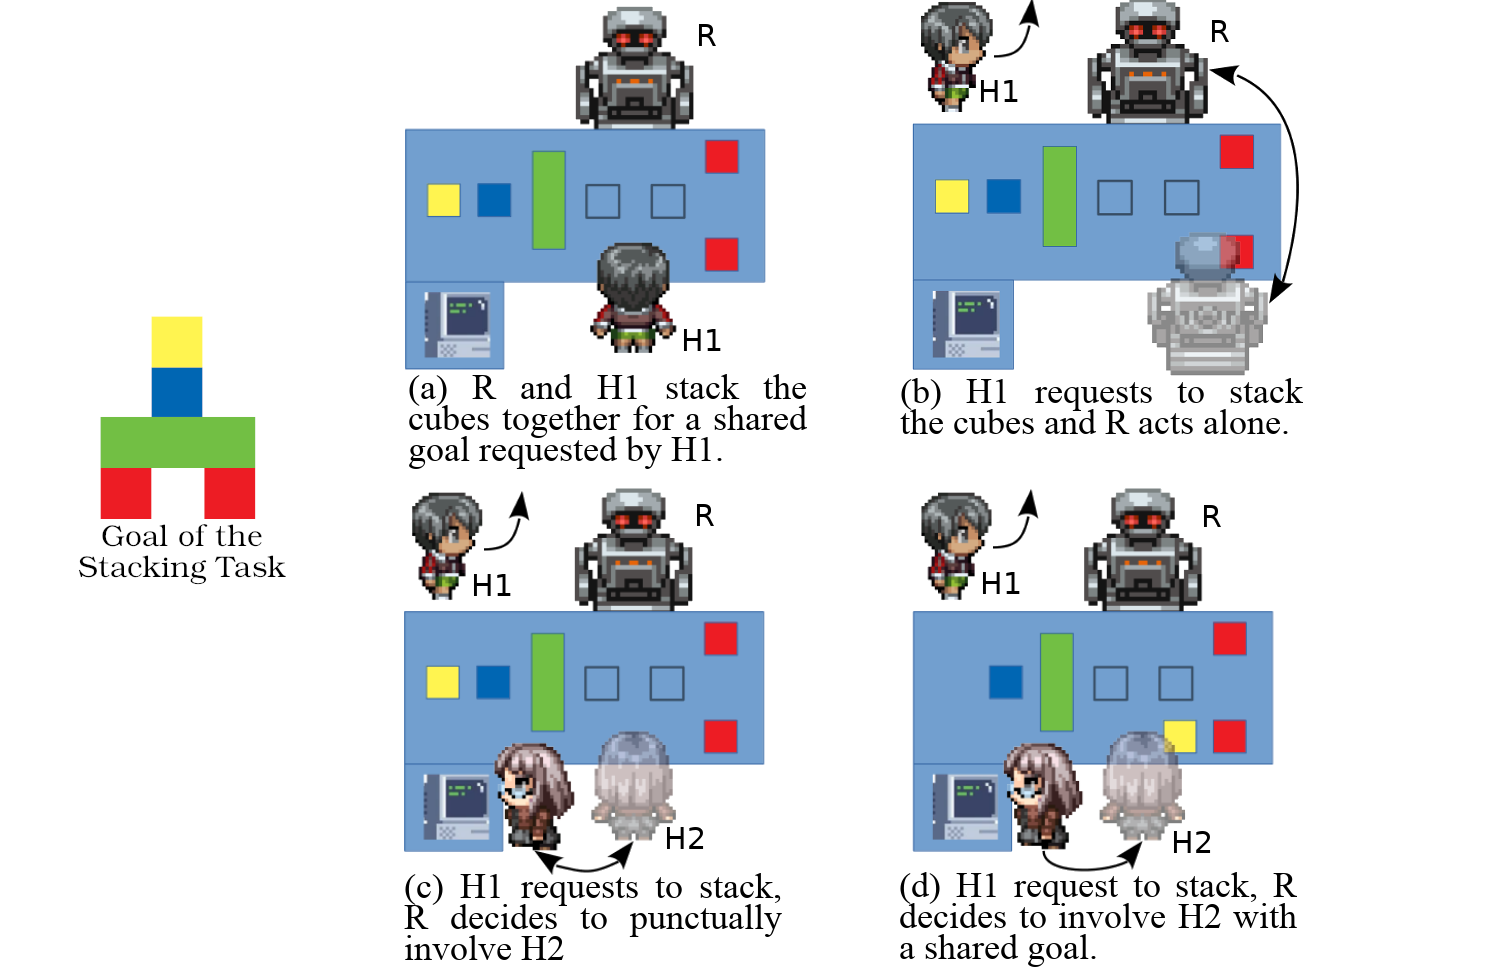
\includegraphics[width=\linewidth]{Chapter2/scenarios.png}
    \caption{Cube stacking scene: A different plan is selected for each scenario, involving nearby humans in the least disturbing way possible}.
    \label{fig:scenarios}
\end{figure}

To highlight the potential of our approach, we present a cube-stacking scene as an example. The scene is depicted in four different scenarios in \ref{fig:scenarios}. The goal consists of stacking the colored cubes on the empty marks to match the colors on the figure's left. All cubes placed in the middle of the table are reachable from anywhere. However, when close to one side, a cube is only reachable from this specific side. Notice that one of the required red cubes is located on the opposite side of the table and cannot be grabbed by the robot in the initial state.

A first human, called \textit{H1}, requests the robot to stack the colored cubes to match the goal pattern given. In the first case (a), \textit{H1} set a shared collaboration goal by requesting the robot to stack the cubes together with them. However, \textit{H1} can also just give their request to the robot and leave. In such a case, the robot has three possibilities. First, in (b), the robot can solve the task alone but must move to the other side of the table, which is slow and costly. Secondly, in (c), the robot can ask another nearby human, \textit{H2}, for punctual help with the unreachable red cube. \textit{H2}'s reaction can be to put the red cube directly in the stack or only make it reachable to the robot. Finally, the robot can set a shared goal by requesting \textit{H2} to help it build the stack together. 

The HATP/EHDA approach explores and evaluates all these kinds of scenarios to produce the robot policy.


\section{Formalization of the Approach}

This section describes the formalization introduced by the HATP/EHDA planning approach and used or adapted in my contributions. It includes descriptions of the problem specifications and the solution produced by the planner.  

\subsection*{Problem Specification}
\label{sec:problem_spec}

The notations from Buisan's thesis have been adapted to match the notations in this thesis and ease readers' comprehension. We start from the classical planning formalization described in~\cite{ghallab2016automated}.

\begin{definition}
    \textbf{(Classical Planning Domain $\Sigma$.)} A \emph{classical planning domain} is a state-transition system in the following form: $\Sigma = (S, A,\gamma)$. $S$ is a finite set of \emph{states} in which the system may be, $A$ is a finite set of \emph{actions} that the agents may perform, $\gamma: S \times A \rightarrow S$ is a \emph{state-transition function}. Each \emph{state} $s \in S$ is a description of the properties of various objects in the planner's environment. 
    \label{def:classical_planning_domain}
\end{definition}

To represent the objects and their properties, we will use two sets $B$ and $X$: $B$ is a set of names for all the objects, plus any mathematical constants representing the properties of those objects. $X$ is a set of syntactic terms called state variables, s.t. the value of each $x \in X$ depends solely on the state $s$.

\begin{definition}
    \textbf{(State-variable $x$.)} A \emph{state-variable} over $B$ is a syntactic term $x = sv(b_1, ..., b_k)$, where $sv$ is a symbol called the state variable's name, and each $b_i$ is a member of $B$ and a parameter of $x$. Each \emph{state-variable} $x$ has a range, $\textit{Range}(x) \subseteq B$, which is the set of all possible values for $x$.
    \label{def:state_variable}
\end{definition}



Here is the description of the sets $B$ and $X$ for the stacking example given in the introduction:
{\small
\begin{align*}
&B           = Entities \cup Locations \cup Reachability \cup Booleans \cup \{\textsf{nil}\} \\
&\quad Entities    = Agents \cup Cubes\\
&\quad Agents      = \{ \textsf{R}, \textsf{H} \} ~~ \backslash\backslash~\textsf{R}:robot,~\textsf{H}:human\\
&\quad Cubes     = \{ \textsf{red1}, \textsf{red2}, \textsf{green1}, \textsf{blue1}, \textsf{yellow1} \}\\
&\quad Locations     = \{ \textsf{base1}, \textsf{base2}, \textsf{bridge}, \textsf{top1}, \textsf{top2} \}\\
&\quad Reachability     = \{ \textsf{middle}, \textsf{sideH}, \textsf{sideR} \}\\
&\quad Booleans    = \{ \textsf{true},\textsf{false} \}\\
&\\
&X = \{ at(e), holding(a), solution(l) ~ | ~ e \in Entities, \agent \in Agents, l \in StackLocations\}\\
&\quad \textit{Range}(holding(\agent) ~|~ \agent \in Agents) = Cubes \cup \{\textsf{nil}\} \\
&\quad \textit{Range}(at(\agent) ~|~ \agent \in Agents) = \{ \textsf{sideH}, \textsf{sideR} \}\\
&\quad \textit{Range}(at(c) ~|~ c \in Cubes) = Reachability \cup Locations\\
&\quad \textit{Range}(solution(l) ~|~ l \in StackLocations) = Cubes \\
\end{align*}
}

% \vspace{-1cm}


\begin{definition}
    \textbf{(Variable value assignment function $\valf$.)} A \emph{variable value assignment function} over $X$ is a function $val$ that maps each $x_k \in X$ into a value $z_j \in$ $\textit{Range}(x_k)$.
    With $X = \{ x_1, ..., x_n \}$, this function can be written as a set of assertions: $\valf = \{ x_1=z_1, \ldots, x_n=z_n \}$. 
    For legibility purposes, we use the following notation to access the value $z_j$ of a state-variable $x_k$ in the state $s_i$: $\valf[][i](x_k) = z_j$.
    \label{def:variable_value_assignment_function}
\end{definition}


\begin{definition}
    \textbf{(Action $a$.)} An \emph{action} is a tuple $a = (\textit{head}(a), \textit{pre}(a), \textit{eff}(a))$ where $\textit{head}(a)$ is a syntactic expression of the form $\textit{act}(z_1, ..., z_k)$ where $act$ is a symbol called the \emph{action name} and $z_1,...,z_k$ are variables called parameters. $\textit{pre}(a) = \{ p_1, ..., p_m \}$ is a set of preconditions, each of which is a literal. And $\textit{eff}(a) = \{ e_1, ..., e_n \}$ is a set of effects, each of which is an expression of the form: $sv(t_1, ..., t_j) \leftarrow t_0$ with $t_0$ being the value to assign to the state variable $sv(t_1, ..., t_j)$. We note $\textit{agt}(a)$ the agent performing the action $a$.
    \label{def:action}
\end{definition}


The problem specification of HATP/EHDA is a pair of two distinct human and robot models as follows: $\mathcal{P} = \{ \agentmodel[H], \agentmodel[R] \}$. Each model $\agentmodel[\agent]$, for an agent $\agent$, comprises the following:
\begin{itemize}
    \item \textbf{Name} ($name^{\agent}$): being the name of the agent. Hence, either ``robot'' or ``human''.
    
    \item \textbf{Beliefs} ($\valf[\agent]$): estimation of the world state from the agent's perspective.
    
    \item \textbf{Agenda} ($\agenda[\agent]$): capturing the personal and/or shared goals of the agent, currently implemented as a task list/sequence but could be generalized to partially ordered task networks.
    
    \item \textbf{Partial Plan} ($\partialplan[\agent]$): storing the current partial plan on an agent. This is empty at the beginning and filled during the planning process.
    
    \item \textbf{Action Model} ($\Lambda^{\agent}$): encoding the capabilities of the agent and used to estimate the next actions of the agent according to their agenda and beliefs. Here, it is described by a \acrfull{htn} and thus a set of operators and methods. 
    
    \item \textbf{Triggers} ($Tr^{\agent}$): describes the reactions the agent may have which might update their agenda. The agent may react to a specific world state, event sequence, or explicit communication. For instance, consider a scenario where another agent is suddenly handing over an object to the agent. This event has nothing to do with the agent's goal, and thus, the next agent action extracted from the Action Model might not consider the other agent. However, a natural reaction to this situation is to grab the handed object. Thanks to the Triggers mechanic, we can model and predict that whatever the agent is doing, the agent will grab the object when given.  
\end{itemize}

Note that most of the models' elements are static during the planning process. Only the Beliefs ($\valf[\agent]$), the Agenda ($\agenda[\agent]$) and the Partial Plan ($\partialplan[\agent]$) of each agent evolve during the planning process. 
That is why we define specifically an \textbf{agent state} in Definition~\ref{def:agent_state}.

\begin{definition}
    \label{def:agent_state}
    \textbf{(Agent state $\agentstate$.)} An \emph{agent state} $\agentstate[\agent]$ comprises the dynamic information evolving during the planning process about an agent $\agent$. It consists of the agent's beliefs, agenda, and partial plan. Hence, the \emph{agent state} is written as follows: $\agentstate[\agent] = \{ \valf[\agent], \agenda[\agent], \partialplan[\agent] \}$.
\end{definition}

\begin{definition}
    \textbf{(Agent model $\agentmodel$.)} An \emph{agent model} $\agentmodel[\agent]$ comprises all information regarding an agent $\agent$. It consists of the static information, such as the agent's name, action model, and triggers, and the dynamic information gathered in the \emph{agent state}. Hence,  an \emph{agent model} is formalized as $\agentmodel[\agent] = \{ name^{\agent}, \Lambda^{\agent}, Tr^{\agent}, \agentstate[\agent], \}$.
    \label{def:agent_model}
\end{definition}

The planner uses two agent models, one for the human and one for the robot. Despite their identical structure, the two models have a fundamental difference: one is a controllable agent and not the other. Indeed, the human model is only used to speculate on human decisions and actions in given situations. 
Then, the robot model is used to plan the robot's actions according to the estimated human actions.
Note that human decisions can still be influenced by the robot's actions, but they cannot be compelled.
It is also important to remember that the two agents are not equivalent. The robot's role is to help, assist, and facilitate humans. Therefore, it should exhibit pertinent, legible, and acceptable behavior.

\begin{definition}
    \textbf{(State $s$.)} A \emph{state} $s_i \in S$ is a tuple composed of two \emph{agent states} capturing the state in which the planning problem is, s.t. $s_i = ( \agentstate[H][i], \agentstate[R][i] )$.
    \label{def:state}
\end{definition}
 

From the robot's perspective, the state of the world is captured by the variable value assignment function $\valf[R][i] \in \agentstate[R][i]$. Since the planner is assumed to be part of the robot, the robot's beliefs are assumed to be the ground truth and are sometimes noted as $\valf[][i]$. 
Similarly, $\valf[H][i] \in \agentstate[H][i]$ represents the estimation of $val_i$ from the human's perspective, also called the estimated human beliefs. 
Therefore, we can define estimated human \textbf{false belief} in Definition~\ref{def:false_belief}.

\begin{definition}
    \textbf{(False belief.)} We say that a state $s_i \in S$ contains \emph{false beliefs}, or \emph{belief divergences}, if $\exists x_j \in X, \valf[H][i](x_j) \neq \valf[R][i](x_j)$. 
    \label{def:false_belief}
\end{definition}


Be careful not to confuse \textbf{\textit{states}} and \textbf{\textit{beliefs}}. A \textit{state} is a state in which a given planning problem is. It comprises the robot and human \textit{agent states}. Each \textit{state} is connected to another through agent actions. On the other hand, the \textit{beliefs} refer to the state of the world from an agent's perspective. Both human and robot \textit{beliefs} are part of a \textit{state}.



As an example, considering the presented stacking example, the associated initial state $s_0$ would be as follows: 

{\small
\begin{align*}
&s_0 = \{\agentstate[R][0], \agentstate[H][0]\} \\
&\quad \agentstate[R][0] = \{ \valf[R][0], \agenda[R][0], \partialplan[R][0] \}, \quad \agentstate[H][0] = \{ \valf[H][0], \agenda[H][0], \partialplan[H][0] \} \\
&\quad \agenda[R][0] = ( Stack ), \quad \agenda[H][0] = \varnothing \\
&\quad \partialplan[R][0] = \partialplan[H][0] = \varnothing \\
&\quad \valf[R][0] = \valf[H][0] = \{ at(\textsf{R}) = at(\textsf{red1}) = \textsf{sideR}, \\
&\quad \quad \quad \quad \quad \quad \quad \quad at(\textsf{H}) = at(\textsf{red2}) = \textsf{sideH}, \\
&\quad \quad \quad \quad \quad \quad \quad \quad at(\textsf{green1}) = at(\textsf{blue1}) = at(\textsf{yellow1}) = \textsf{middle}, \\
&\quad \quad \quad \quad \quad \quad \quad \quad holding(\textsf{R}) = holding(\textsf{H}) = \textsf{nil}, \\
&\quad \quad \quad \quad \quad \quad \quad \quad solution(\textsf{base1}) = solution(\textsf{base2}) = \textsf{red}, \\
&\quad \quad \quad \quad \quad \quad \quad \quad solution(\textsf{bridge}) = \textsf{green},   \\
&\quad \quad \quad \quad \quad \quad \quad \quad solution(\textsf{top1}) = \textsf{blue}, \\
&\quad \quad \quad \quad \quad \quad \quad \quad solution(\textsf{top2}) = \textsf{yellow} \}  \\
\end{align*}
}

Note that our model permits interaction with only one human at a time. Hence, in scenario (a) on figure~\ref{fig:scenarios}, $\agentmodel[H]$ corresponds to \textit{H1}. In all other scenarios, \textit{H1} only initializes the robot's agenda. Thus, in such cases, $\agentmodel[H]$ corresponds to \textit{H2}.
Therefore, $d^H_0$ is empty except in scenario (a), where \textit{H1} establishes a shared goal. Also, the sets $B$ and $X$ have been slightly modified for legibility reasons because the cubes are, in fact, explicitly associated with colors used in the task decompositions. As a result, the solution is expressed using colors and not the cube names. Finding the exact cube to place is described in the action models.

\subsection*{Planning and Estimating Actions}

As mentioned above, the two models $\agentmodel[R]$ and $\agentmodel[H]$ are fundamentally different. The human one is used to estimate the actions that the human is likely to perform in a given situation. The robot one is used to plan the best robot actions according to the estimated human ones. Nevertheless, to simplify the description, we tend to refer to both cases as ``estimating an agent's next actions''.

The exact process of estimating the next actions that an agent $\agent \in Agents$ is likely to perform in a state $s_i \in S$ will be detailed later. Here, we only consider an overview to introduce some notations. 
The process roughly consists of using the agent's static action model ($\Lambda^{\agent}$) 
and the dynamic agent's beliefs ($\valf[\agent][i]$)
to refine the agent's agenda ($\agenda[\agent][i]$). This refining process returns a so-class \textit{refinement} defined in Definition~\ref{def:refinement}.

\begin{definition}
    \textbf{(Refinement $ref$.)} A \emph{refinement} is a list of 2-tuples for each estimated action, $a$, and the associated new agenda, $d$, after being refined, s.t., $ref(\agenda[\agent][i], \valf[\agent][i]) = \{ (a_1,\agenda[]1), ..., (a_k,\agenda[]k) \}$. It is computed using the agent's action model $\Lambda^{\agent}$.
    \label{def:refinement}
\end{definition}


In our cooking example, we obtain the following refinement if the starting agent is the human:

\begin{equation*}
    ref(\agenda[H][0], \valf[H][0]) = \{ (add\_salt(),\agenda[]1), (move\_to(\textsf{kitchen}),\agenda[]2) \}
\end{equation*}

The execution of an action $a$ in HATP/EHDA is seen and known by both agents. Thus, $\forall \agent \in Agents, \forall x \in X$: 
\begin{equation}
    \valf[\agent][i+1](x) = \left\{ 
    \begin{array}{ll}
        w, & \mbox{if} ~ x \leftarrow w \in \textit{eff}(a)   \\ 
        \valf[\agent][i](x), & \mbox{otherwise}
    \end{array}\right.
\end{equation}


\subsection*{Solution description}

HATP/EHDA produces a robot policy extracted from an implicitly coordinated joint solution tree. This solution tree is an AND/OR tree where AND nodes correspond to human decisions, all possible human choices are preserved, and each OR node corresponds to a robot action selected among the possible robot actions. This representation assumes a turn-taking fashion where agents act one after another alternatively. The solution is formally defined in definition~\ref{def:joint-sol-plan}.

\begin{definition} 
    \label{def:joint-sol-plan}
    \textbf{(Implicitly Coordinated Joint Solution.)} 
    {The solution for $P$ is represented as a tree, i.e. $G=(V,E)$. Each vertex ($v \in V$) represents the robot's belief state, starting from the initial belief. Each edge ($e \in E$) represents a primitive task that is either a robot's action $a^{r}$ or a human's estimated and emulated action $a^{h}$. $G$ gets branched on the possible choices ($a^{h}_1$, $a^{h}_2$, ..., $a^{h}_m$). 
    }  
    \end{definition}
    
In practice, it produces a tree of sequential actions where every human action is succeeded by one optimal robot action. Additionally, a new branch is created for every estimated possible human action, ensuring it covers all possible human choices. Each branch is a possible course of alternating robot and human actions leading to the goal.
Each branch in the solution tree is a sequence of primitive actions, say $\pi=(a_1^h,a_2^r,a_3^h,...,a_{k-1}^h,a_k^r)$, that must satisfy all the solution conditions of $\mathcal{P}$. 
Here, each $a_i^h$ represents a choice, often out of several, the human could make. And each $a_{i+1}^r$ is the optimal robot action according to $a_i^h$.


\section{Exploration and Search Process}

To start planning, HATP/EHDA must be given the two action models (the robot and the human HTNs), the initial beliefs of both agents (which can differ), and the initial agenda of both agents. The initial agenda of the robot represents the task to decompose, while the agenda of the human represents any task the human is estimated to be committed to. If a shared goal has been established prior to planning between the robot and the human (\textit{e.g.}, the human asking to perform a task with the robot), the agenda of both agents will be filled with the same task.

The planning process is done in three parts: (1) both HTNs are explored in a turn-taking fashion, resulting in a valid joint plans tree; (2) based on this tree, robot actions are selected according to action, plan-wide and social costs, resulting in a conditional plan, where at each step multiple human actions can be performed but only one robot action is set; (3) causal and threat links are added between actions of the conditional plan to ease its execution.

The robot HTN exploration is a pretty standard depth-first algorithm. The first task $\lambda$ from its agenda $d^R$ is popped, then if it is an abstract task $\lambda \in Ab$, all the applicable methods are applied, and their results are prepended to the agenda, thus giving new agents state (with the same beliefs as the previous ones but with the robot agenda updated) and branching our search space. We recursively iterate with the new task popped from the new robot agenda. Eventually, the popped task will be a primitive one $\lambda \in Op$, and its function will be applied to the currently explored agent states. If it returns \textit{false} ($\bot$), the action is not applicable, and the exploration backtracks to another decomposition of an abstract task. However, if the action is applicable, it is added to the robot plan, and the triggers are run for each agent, updating their agenda if necessary. The human \acrshort{htn} is then queried to get their possible next actions from this new state. The possible actions found are added to the human plan, and, for each possible new state, we apply each agent's triggers and then continue the robot \acrshort{htn} exploration. This exploration continues until the robot agenda is empty, or all the branches return \textit{false}. The exploration process is summarized in Fig.~\ref{fig:HATPEHDA_planning_process}.

\begin{figure}
    \centering
    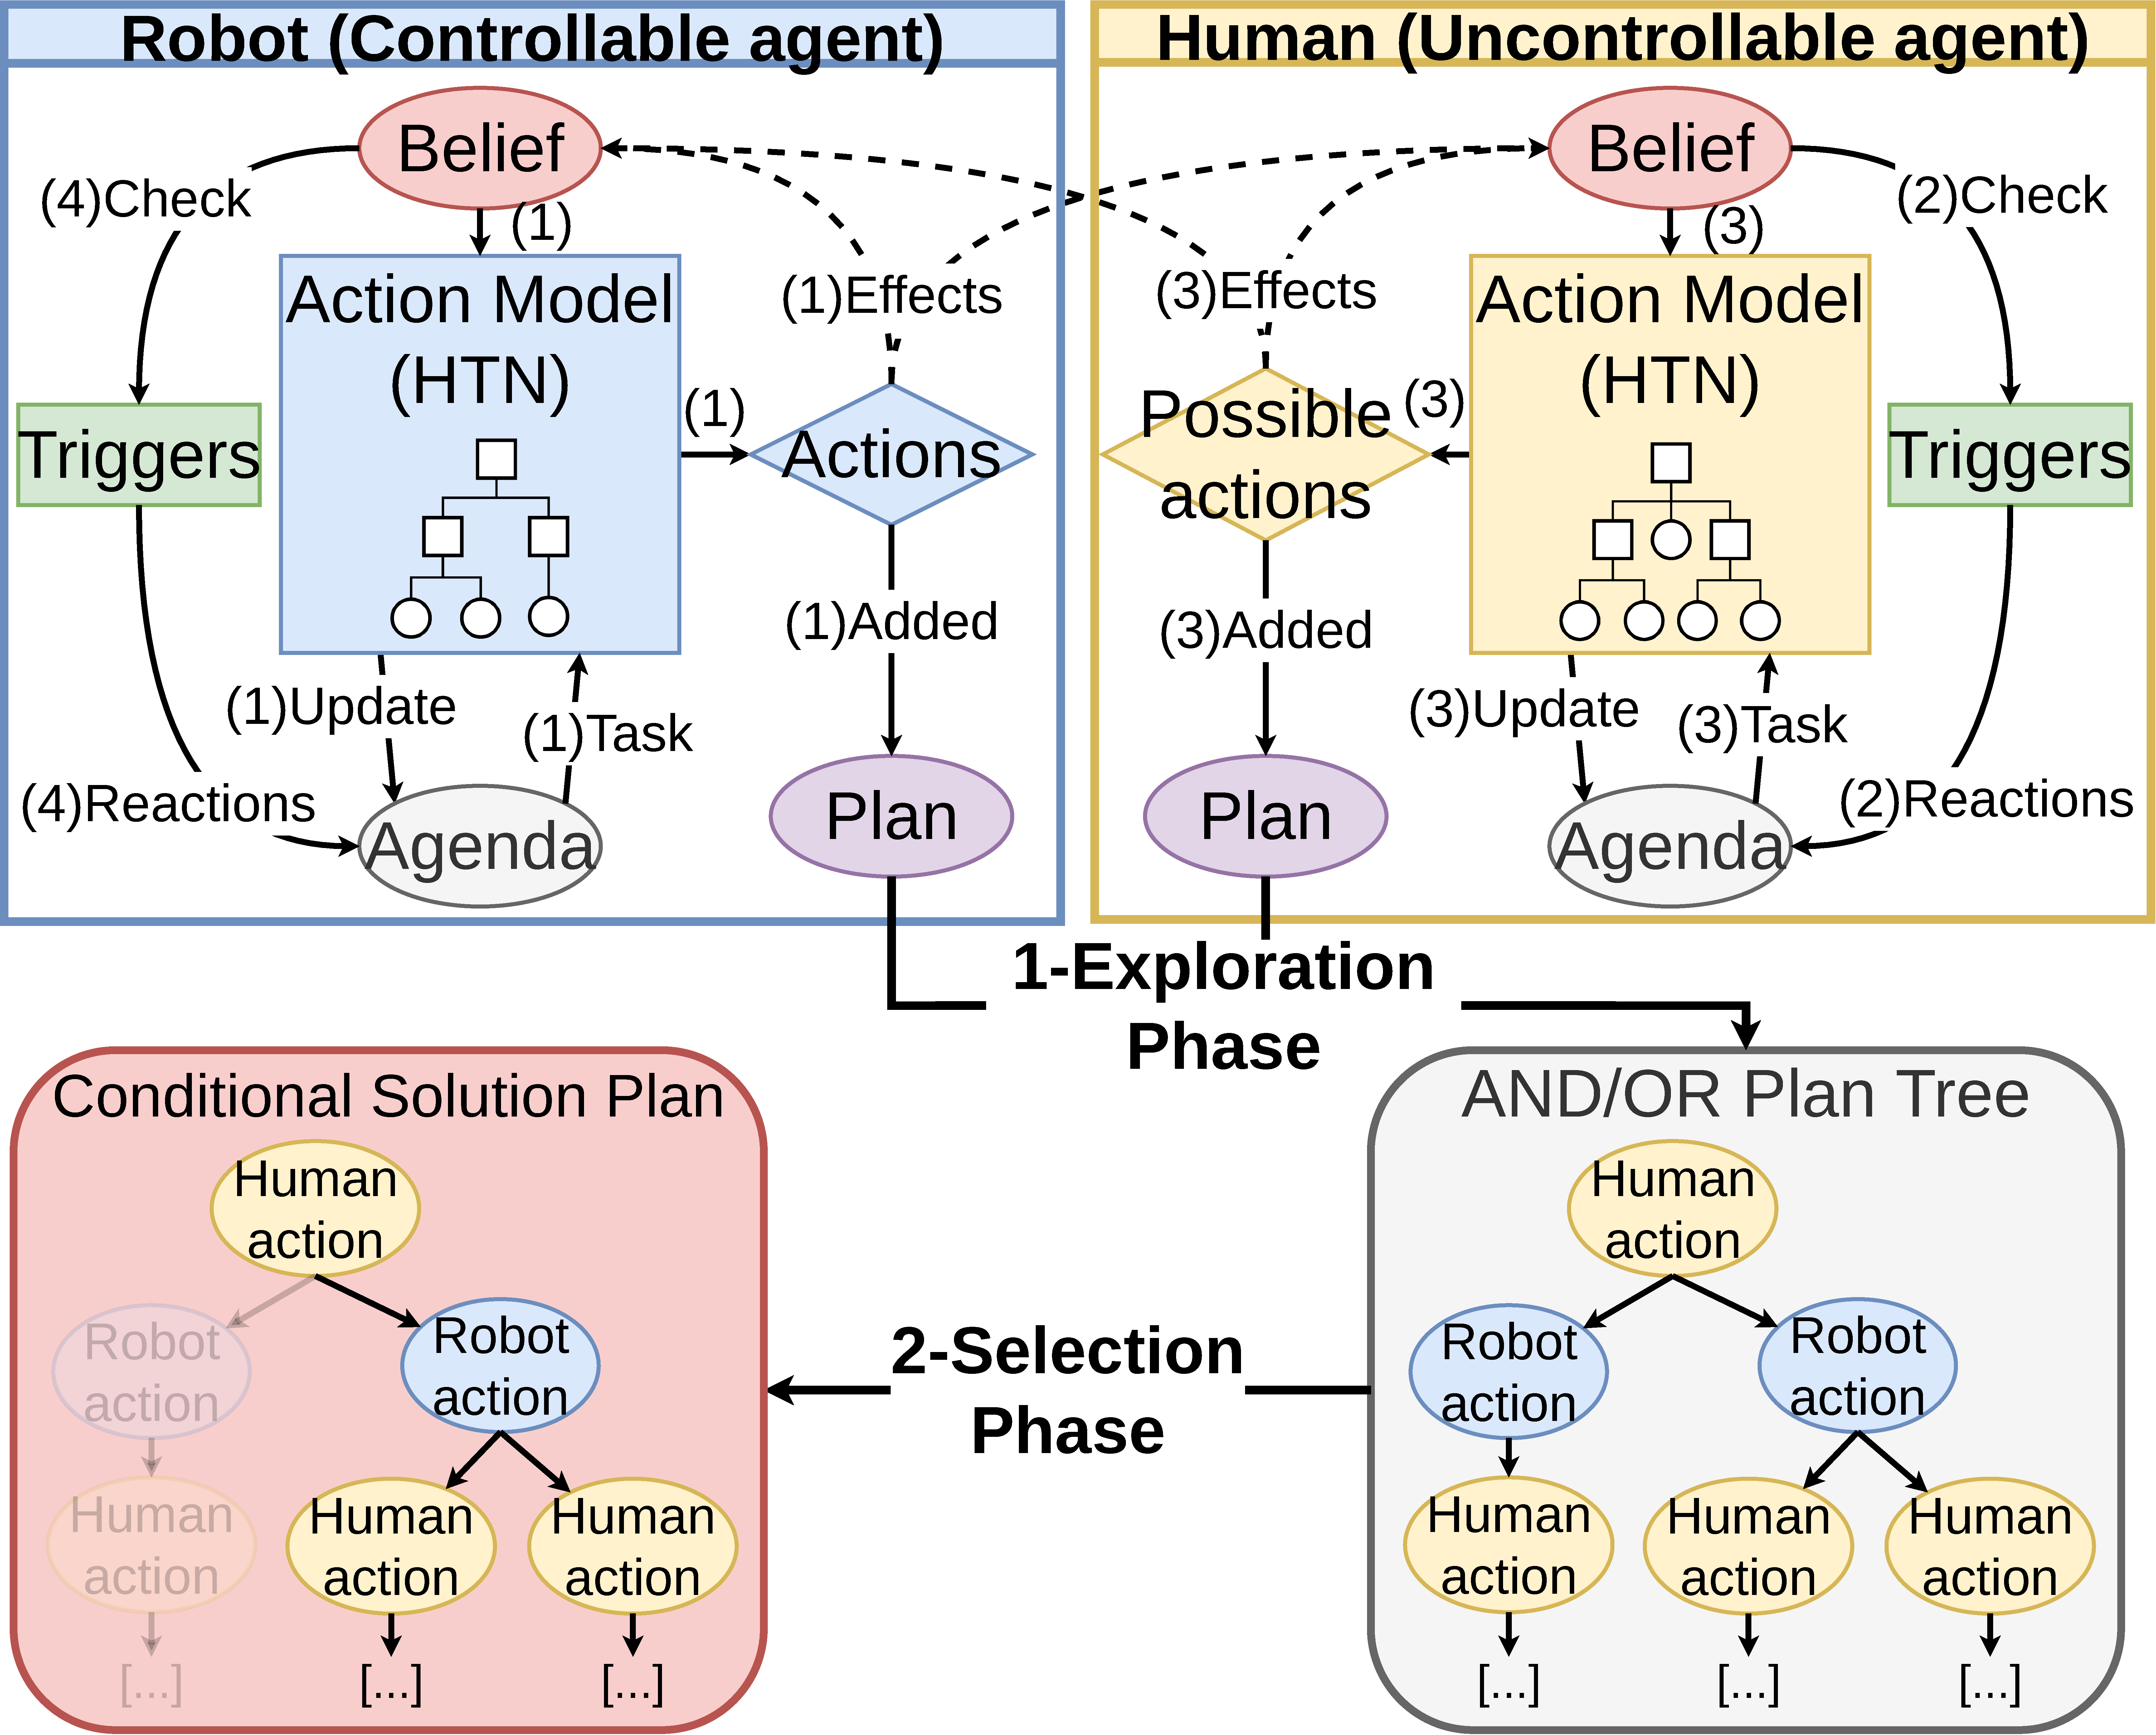
\includegraphics[width=\linewidth]{Chapter2/HATPEHDA_planning_process.pdf}
    \caption{The HTNs exploration consists in iterative loops of four steps : (1) Get possible robot actions from the robot HTN, add them to the plan and apply their specific effects on the H \& R beliefs, (2) Check Triggers and add the reactions in the corresponding agendas, (3) Get possible human actions based on their estimated beliefs, add them in the plan and apply their effects on the H \& R  beliefs, (4) Check Triggers again and add the reactions in the corresponding agendas. Here the robot is starting, but the human could with the following ordering: (3)>(4)>(1)>(2).}
    \label{fig:HATPEHDA_planning_process}
\end{figure}

The human \acrshort{htn} exploration differs from classical \acrshort{htn} planning as the goal is not to produce a complete plan but to list all the actions the human is likely to perform in a given agent state. 
We recursively decompose the first task of the human agenda $d^H$ with every applicable method until we reach an applicable operator. All the operators from all the applicable decompositions are returned to the robot HTN exploration and applied.

Two special cases are handled during the exploration. 
When an agent's agenda is empty, the exploration returns a default passive action \textit{IDLE}, which has no effect. It only indicates that the agent has nothing to do and will likely remain still. 
Besides, if no applicable action is found for an agent, the exploration returns a default passive action \textit{WAIT}. Similarly to \textit{IDLE}, it has no effect but represents the agent's impossibility to act in the current situation. 

Once both agendas are empty, the state is set as a success, the plan is added to the valid plans tree, and the search can continue until no decomposition is left for any task.


\section{Plan Evaluation and Selection}

In human-aware task planning, plan evaluation is a trade-off between efficiency and social criteria.
The robot should be efficient but also behave in an acceptable, legible, and accommodating manner.  


Cost evaluation is tricky because objective metrics are easy to use for efficiency. However, social criteria are more challenging to evaluate because they are hard to generalize. These social rules can be very context-dependent, making them hard to generalize and thus to take into account reliably.

Plan cost is a mix of all the following:

\begin{itemize}
    \item Length of the plan (number of actions or temporal duration if available).
    \item Sum of individual action cost: the cost of each action can be estimated to translate the effort required to perform it. It can reflect several aspects and constraints, such as pure physical strength required, duration of the action, or energy consumption.
    \item Undesired states: Common sense and social norms can be used to define several rules defining undesired states. This can cover various aspects such as hygiene or safety. For instance, despite being possible and maybe efficient, we would not like a robot holding a dirty dripping mop in one hand and the sandwich we asked for in the other hand. Another example is that we would not like a robot dropping a knife just on the edge of a table or counter because it may fall and be dangerous. 
    \item Undesired sequences of actions: For the same reasons, we can also define undesired sequences of actions. This can express preferences regarding the ordering of different subtasks, \textit{e.g.}, since we do not want the robot to hold our sandwich while cleaning the house, we would also not like the robot to clean first and then make a sandwich because the robot is likely to be dirty while making the sandwich.  
\end{itemize}

I implemented in HATP/EHDA a way to specify and take into account undesired state and action sequences. Detecting any of them in a possible plan would penalize the plan cost of the specified amount. Here, the undesired elements must be specified in the problem specification and are abstracted in the planner. However, as stated above, it is hard to generalize undesired states and action sequences and integrate them directly in the planner to avoid specifying them in the problem specification.

In HATP/EHDA, once the exhaustive exploration has been done, the result is a valid plan tree of alternating feasible robot and human actions along with their current beliefs leading to task completion. This second planning step aims to select robot actions, such as each human action in the plan has only one robot action as a child.
To do so, we define a cost function $cost: S \times Op \mapsto \mathbb{R}^+$ representing the cost of an action in a specific state. The data structure is now similar to a two-player game tree. However, \textit{MinMax} approaches are unsuitable here, as we are not in an adversarial setup but more in a collaborative one. Indeed, trying to minimize the maximum possible cost assumes that humans will always do the actions that lead to the worst plan. This defensive behavior could lead to non-optimal plans. We thus propose to explore this tree differently.

Moreover, like in \acrshort{hatp}, we can define \textit{social costs} functions. These functions take a complete human and robot sequence of actions ($\pi^R$ and $\pi^H$) and return a cost ($\mathbb{R}^+$) which is added to the cost of the plan previously determined. By doing so, we can penalize non-acceptable sequence of robot actions (\textit{e.g.} serving a meal just after taking out the trash) or non-satisfactory human required contribution (\textit{e.g.} the robot requesting the human to perform small tasks multiple times instead of giving the big picture of the actual task to perform).

The approach we propose for plan selection is to minimize the average cost. It represents the human potentially selecting any course of action in their stream (while still respecting the action model defined in their HTN).
The algorithm is given the root action of the plan tree previously generated. It returns the cost of the conditional plan selected while selecting the robot actions in the plan tree to minimize the average plan cost.

\section{Qualitative Results}

Each scenario is commented on below with their corresponding selected plan shown in TABLE~\ref{tab:plans}. The partial robot and human action models and their exploration are presented in Fig.~\ref{fig:plans}.

\begin{table}[h]
\small
\begin{tabularx}{0.98\textwidth}{|X||X|}
    \hline
    \textbf{(a) \textit{R} and \textit{H1} build the stack together as a shared goal requested by \textit{H1}.}     & \textbf{(b) \textit{H1} requests to stack the cubes and \textit{R} acts alone.} \\
    \hline
    R-PickAndPlace(red, base)     & R-PickAndPlace(red, base) \\ 
    H1-PickAndPlace(red, base)     & R-moveTo(red) \\  
    R-PickAndPlace(green, bridge) & R-PickAndPlace(red, base) \\
    H1-PickAndPlace(blue, top)     & R-moveTo(init) \\
    R-PickAndPlace(yellow, top)   & R-PickAndPlace(green, bridge) \\
                                    & R-PickAndPlace(blue, top) \\
                                    & R-PickAndPlace(yellow, top) \\
    \hline \hline
    \textbf{(c) \textit{H1} requests R to build the stack, \textit{R} decides to punctually involve \textit{H2}.} & \textbf{(d) \textit{H1} requests R to build the stack, \textit{R} decides to invite H2 to a shared goal.} \\
    \hline
    R-PickAndPlace(red, base)     & R-PickAndPlace(red, base) \\
    H2-IDLE                        & H2-IDLE \\
    R-AskPunctualHelp(red)        & R-AskSharedGoal() \\
    H2-PickAndPlace(red, base)     & H2-PickAndPlace(red, base) \\
    R-PickAndPlace(green, bridge) & R-PickAndPlace(green, bridge) \\
    H2-IDLE                        & H2-PickAndPlace(blue, top) \\
    R-PickAndPlace(blue, top)     & R-PickAndPlace(yellow, top) \\
    H2-IDLE                        & \\
    R-PickAndPlace(yellow, top)   & \\
    \hline
\end{tabularx}
\caption{Execution trace of a selected plan for each scenario.}
\label{tab:plans}
\end{table}

\begin{sidewaysfigure}
    \centering 
    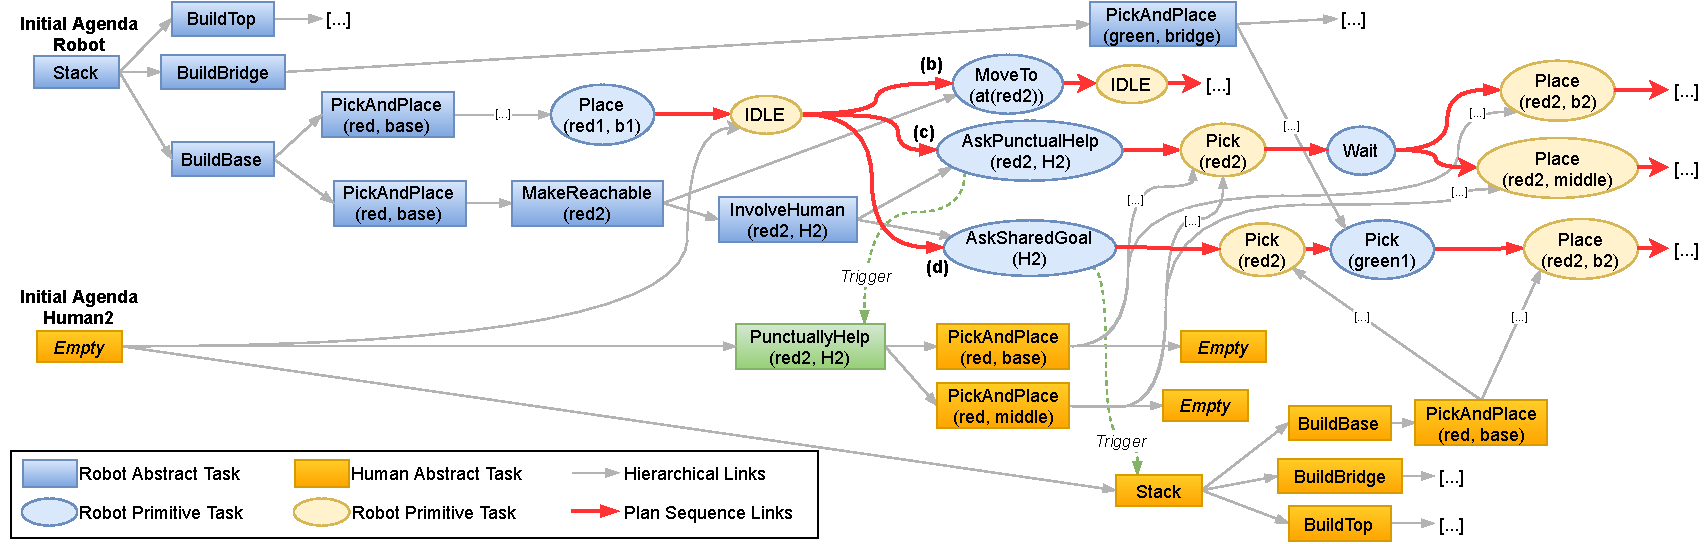
\includegraphics[width=1.0\textwidth]{Chapter2/plans.pdf}
    \caption{Illustration of the incremental exploration of various courses of actions corresponding to scenarios depicted in Fig.~\ref{fig:scenarios}(b), (c), and (d). Since \textit{H1} requests the robot to complete the task without establishing a shared goal, the robot agenda only contains the task to achieve, and the agenda of \textit{H2} starts empty.}
    \label{fig:plans}
\end{sidewaysfigure}

\paragraph{(a) \textit{H1} and R act together}
First, the human sets a shared goal by asking the robot to stack cubes with him. Since it is a shared goal, human and robot agendas are initialized with the ``Stack" task. Thus, the robot anticipates that the human will pick the unreachable second red cube by querying the human action model. Table~\ref {tab:plans}(a) shows the selected plan to collaboratively stack the cubes. 

\paragraph{(b) \textit{R} acts alone}
This time, the human asks the robot to stack the cubes but then leaves the scene, and the robot must act alone. Hence, the only applicable method to make the second red cube reachable is to move to the other side even though the movement action is expensive (we can imagine a table way longer than shown in the figure).

\paragraph{(c) \textit{R} asks punctual help}
The first human (\textit{H1}) requests the robot to complete the task, and another uninvolved human (\textit{H2}) is present. The robot starts exploring its \acrshort{htn} and, thanks to the presence of the other human, a new method is applicable, allowing the robot to ask for help. It can ask for punctual help or a complete commitment of \textit{H2} to the task. Of course, asking for help for one cube is less costly than building the whole stack together. However, asking for help from someone not already involved in a common task is still expensive since they must put themselves in the task's context. 
Nevertheless, this punctual help is less costly for the robot than moving to the other side, so this solution is selected. Note that we model that after being asked to help punctually, the human can either stack the cube themself or make it reachable to the robot by placing it in the middle. Only the first branch is shown in table~\ref{tab:plans}(c), but the selected plan is in fact conditional with two branches as depicted in Fig.~\ref{fig:plans}.

\paragraph{(d) \textit{R} invites \textit{H2} to share a goal}
Same initial setup, but now two cubes are out of reach. Asking for punctual help is still less costly than moving around the table. 
However, each new request to \textit{H2} is assumed to be more and more costly, making repeated queries expensive.  
Therefore, due to the two unreachable cubes in this scenario, setting a shared goal becomes less costly for the robot than asking twice for punctual help.

\section{Conclusion}

What is offered by HATP/EHDA is very interesting. We rely and reason on the human model to plan the robot's actions while never compelling the human actions. The plan produced assumes turn-taking and no parallel execution of the actions. This is not a strict constraint as a post-analysis can reason on the causal links of the actions in the plan to extract a partially ordered plan to execute, making the execution more flexible. However, It is still a limitation addressed in Chapter~\ref{chap:4}.